% Defense slide (after VD2): extracting the true bulk tensor.
% Left: e^{tau H} built on FIVE sites, so the centre tensor has every NNN
% partner inside; that centre tensor (highlighted) is the one extracted.
% Right: after the rotation it is repeated as the transfer-matrix column.
\documentclass[tikz,border=3pt]{standalone}
\usepackage{amsmath,amssymb,braket}
\usetikzlibrary{arrows.meta}

\definecolor{tnE}{RGB}{250,200,70}
\definecolor{tnbnd}{RGB}{196,98,22}
\definecolor{tncool}{RGB}{240,224,178}

\begin{document}
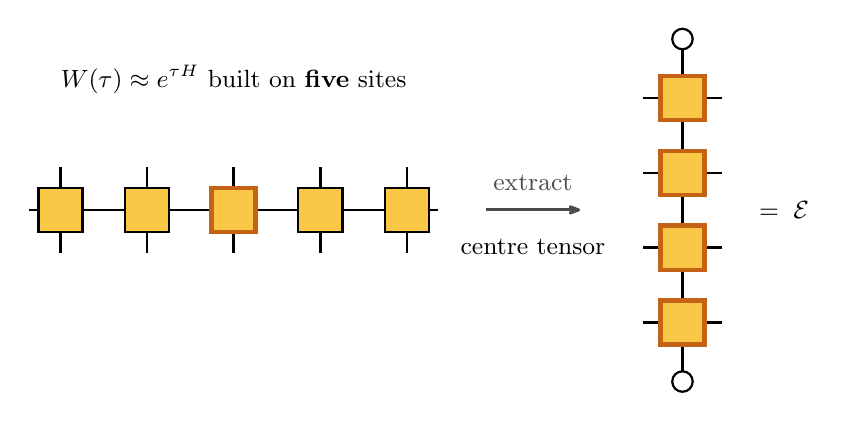
\begin{tikzpicture}[
    >={Stealth[round,length=2.2mm]},
    bond/.style={draw=black, line width=0.9pt},
    W/.style={rectangle, draw=black, line width=0.9pt, fill=tnE, minimum size=5.6mm, inner sep=0pt},
    Wc/.style={rectangle, draw=tnbnd, line width=1.6pt, fill=tnE, minimum size=5.6mm, inner sep=0pt},
    P/.style={circle, draw=black, line width=0.8pt, fill=white, minimum size=2.6mm, inner sep=0pt},
    tag/.style={font=\small},
  ]

  %% ---------------- left: W(tau) on five sites ----------------
  \node[tag, anchor=south] at (2.2,1.35) {$W(\tau)\approx e^{\tau H}$ built on \textbf{five} sites};
  \draw[bond] (-0.4,0) -- (4.8,0);
  \foreach \i in {0,...,4} {
    \draw[bond] ({\i*1.1},0.0) -- ({\i*1.1},0.55);
    \draw[bond] ({\i*1.1},0.0) -- ({\i*1.1},-0.55);
  }
  \foreach \i in {0,1,3,4} { \node[W] at ({\i*1.1},0) {}; }
  \node[Wc] at (2.2,0) {};

  %% ---------------- arrow ----------------
  \draw[->, line width=1.1pt, black!70] (5.4,0) -- (6.6,0)
    node[midway, above=3pt, tag] {extract};
  \node[tag, anchor=north] at (6.0,-0.25) {centre tensor};

  %% ---------------- right: repeated as the transverse column ----------------
  \begin{scope}[xshift=7.9cm, yshift=-1.98cm]
    \draw[bond] (0,-0.20) -- (0,4.15);
    \foreach \j in {0.55,1.50,2.45,3.40} {
      \draw[bond] (-0.5,\j) -- (0.5,\j);
      \node[Wc] at (0,\j) {};
    }
    \node[P] at (0,-0.20) {};
    \node[P] at (0,4.15) {};
    \node[tag, anchor=west] at (0.85,1.975) {$=\;\mathcal{E}$};
  \end{scope}

\end{tikzpicture}
\end{document}
